Questa sezione descrive il processo di sviluppo adottato nell\rq ambito del progetto \emph{GoBus}.

\subsection{Modello del Ciclo di Vita}
Il ciclo di vita è stato scelto in base alle tempistiche e agli obiettivi del progetto. In particolare, considerata la necessita di comprendere meglio i requisiti che il committente richiedeva \`{e} stato scelto un modello \emph{evolutivo a prototipazione}. Questo modello consente di fornire al committente un prototipo del sistema in tempi rapidi. La scelta di questo modello \`{e} stata dettata dalle caratteristiche del progetto da realizzare, ovvero:
\begin{itemize}
\item dalla sua natura interattiva;
\item dall\rq importanza dell\rq usabilit\`{a};
\item dalle dimensioni poco estese;
\item dalla struttura altamente modularizzata che prevede bassi costi di manutenzione.
\end{itemize}
L\rq uso di questo modello permette di avere feedback periodici utili per la continuazione delle attivit\`{a} progettuali.

\subsection{Requirement Elicitation and Analysis}
La fase di requirement elicitation consiste nella comprensione delle necessit\`{a} del committente al fine di collezionare i requisiti del sistema. Nell\rq ambito del progetto, tale attivit\`{a} \`{e} stata svolta facendo brainstorming con tutti gli stakeholder interessati. In particolare, sono stati organizzati incontri sia con i coordinatori del progetto sia con aziende di trasporto locali. Per mitigare il richio di errata comprensione delle reali necessit\`{a} degli stakeholder, i meeting si sono ripetuti cos\`{i} che, ad ogni incontro, i requisiti potessero essere meglio fissati. Il numero totale di incontri tenuti con gli stakeholder \`{e} stato pari a tre.\\
La tabella \ref{tab:gestioni} mostra, ad alto livello, i principali raggruppamenti di funzionalità identificati nell'ambito del progetto \emph{GoBus}. Di seguito ognuno di essi verr\`{a} analizzato in dettaglio. Si noti che per evitare ridondanza e per ragioni di spazio, non sono riportati tutti i requisiti funzionali identificati. Per la lista completa, si faccia riferimento al Documento di Analisi dei Requisiti (RAD) in allegato.\\

\begin{table*}[tb]
   \centering
   \caption{Overview delle Funzionalit\`{a} Identificate}
   \label{tab:gestioni}
  \resizebox{1\linewidth}{!}{
   \begin{tabular}{ll}\hline
   Nome & Descrizione\\\hline
   Gestione Registrazione & Insieme di funzionalit\`{a} che consentono la registrazione di un nuovo utente.\\
   Gestione Autenticazione & Insieme di funzionalit\`{a} che consente il riconoscimento degli utenti registrati.\\
   Gestione Account & Insieme di funzionalit\`{a} per la manipolazione degli account degli utenti.\\
   Gestione Fermate & Funzionalit\`{a} che consente di visualizzare le fermate tramite l\rq applicazione di diversi filtri per la ricerca mirata.\\
   Gestione Linee & Funzionalit\`{a} che consente la visualizzazione delle linee tramite l\rq applicazione di diversi filtri per la ricerca mirata.\\
   Gestione Percorso & Insieme di funzionalit\`{a} che consente la visualizzazione delle indicazioni stradali.\\
   Gestione Preferiti & Funzionalit\`{a} che consente la gestione delle fermate e delle linee preferite.\\
   Gestione News & Insieme di funzionalit\`{a} per la efficace gestione degli avvisi da parte delle aziende di trasporti.\\
   Gestione Dati GTFS & Insieme di funzionalit\`{a} che consente ad un\rq azienda di trasporti di caricare il proprio file GTFS.\\
   \hline
   \end{tabular}
   }
\end{table*}

\noindent {\bf{Gestione Registrazione}}: permette ad un nuovo utente di iscriversi alla piattaforma. Si noti che ci sono diverse modalità di registrazione:
\begin{itemize}
\item utilizzando la propria e-mail, fornendo un nickname ed una password;
\item tramite il proprio account Facebook;
\item tramite il proprio acccount Google.
\end{itemize}
I requisiti della gestione registrazione sono comuni sia all'applicazione web che all'applicazione mobile.
\noindent {\bf{Gestione Autenticazione}}: Questa gestione permette ad un utente registrato di essere riconosciuto e abilitato a effettuare determinate operazioni da parte del sistema. Fanno parte di questa gestione anche le funzionalit\`{a} di login e logout.\\

\noindent {\bf{Gestione Account}}: si occupa di tutto ci\`{o} relativo alla manipolazione delle informazioni personali degli utenti registrati al sistema. Nel dettaglio, l'utente può visualizzare i dettagli del suo account, modificarli o rimuovere il suo account dalla piattaforma.\\

\noindent {\bf{Gestione Fermate}}: permette di visualizzare le fermate applicando pi\`{u} filtri, in modo da effettuare ricerche mirate alle necessità dell'utente. \`{E} possibile visualizzare le fermate:
\begin{itemize}
\item utizzando i dati geografici dell'utente;
\item filtrando per località;
\item filtrando per azienda di trasporto.
\end{itemize}
\`{E} possibile, inoltre, visualizzare le linee relative ad una fermata per consentire all'utente di conoscere le linee che l'attraversano.\\

\noindent {\bf{Gestione Linee}}: permette di visualizzare le linee tramite l\rq applicazione di pi\`{u} filtri in modo da effettuare ricerche mirate alle necessità dell'utente. \`{E} consentita la visualizzazione delle linee di una specifica localit\`{a}. Per ogni linea \`{e} possibile conoscerne i dettagli e visualizzare gli orari delle relative corse. Inoltre, \`{e} possibile visualizzare l'intero percorso di una corsa.\\

\noindent {\bf{Gestione Percorso}}: permette all'utente di ottenere informazioni circa il percorso da seguire, ovvero le soluzioni che gli permettano di raggiungere la destinazione scelta.\\

\noindent {\bf{Gestione Preferiti}}: permette all'utente di memorizzare le corse, linee, e citt\`{a} a cui accede pi\`{u} frequentemente.\\

\noindent {\bf{Gestione News}}: permette all'utente di essere informato sulle modifiche relative al servizio di trasporto pubblico. Le aziende possono, in tempo reale, aggiungere notizie, modificarle e eliminarle. Questa funzionalit\`{a} \`{e} stata implementata esclusivamente per la web application.\\

\noindent {\bf{Gestione dati GTFS}}: consente ad una azienda di trasporti di poter caricare le informazioni relative al proprio servizio, tramite file del formato GTFS. Questa funzionalit\`{a} \`{e} stata implementata all'interno della web application.\\

L'analisi dei requisiti \`{e} poi proseguita tramite i casi d\rq uso. In seguito, verr\`{a} mostrato lo sviluppo di una funzionalit\`{a} a partire dal requisito funzionale fino alla fase di testing in modo da consentire al lettore di comprendere la metodologia di modellazione adottata. In dettaglio, il requisito preso in considerazione \`{e} quello relativo alla ricerca di una linea.

\begin{figure*}[tb]
\centering
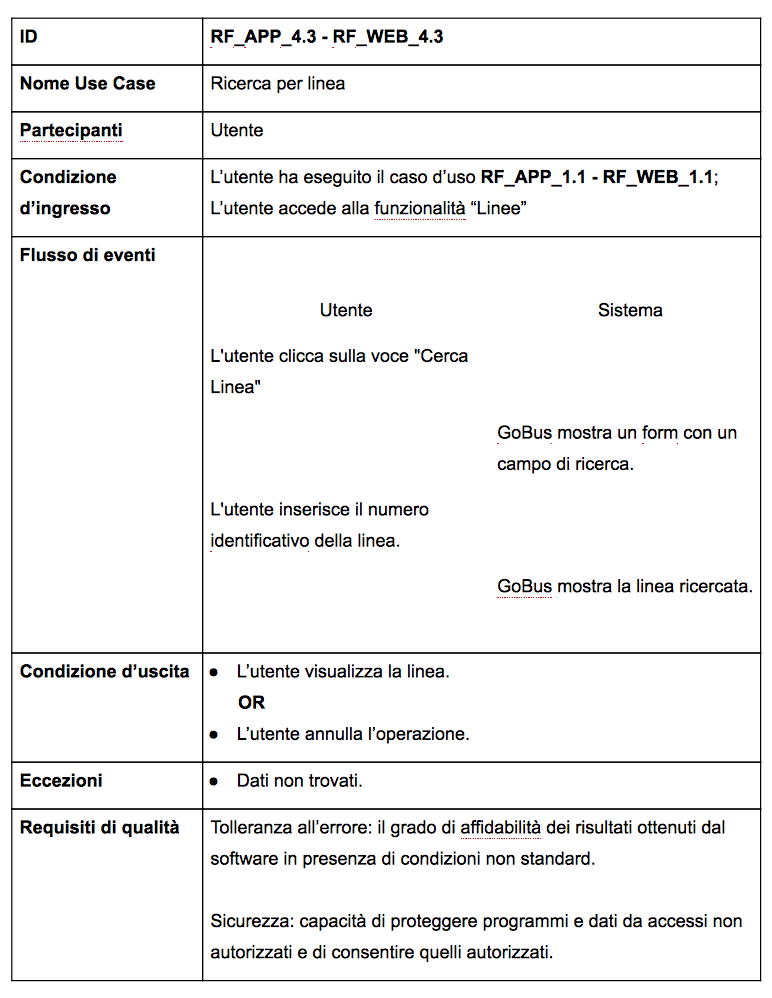
\includegraphics[scale=.7]{img/cd.png}
\caption{Caso d\rq uso relativo al requisito funzionale che consente la ricerca di una linea.}
\label{fig:cd}
\end{figure*}

La Figura \ref{fig:cd} mostra il caso d\rq uso relativo al requisito funzionale che consente la ricerca di una linea. In particolare, l'utente registrato, dopo aver effettuato l'accesso al sistema (condizione d\rq entrata necessaria), clicca sul tasto che consente la ricerca di una linea e inserisce i dati necessari. Il sistema accede alla base di dati e carica i dati relativi alla linea ricercata. Si noti che ogni caso d\rq uso del sistema modella un requisito sia considerando le azioni che intercorrono tra l\rq utente e il sistema, sia considerando i requisiti di qualit\`{a} e le eventuali condizioni che potrebbero causare eccezioni.\\

Il successivo passo nella modellazione delle funzionalit\`{a} del sistema \`{e} consistito nella definizione dei path navigazionali relativi a ciascun raggruppamento di requisiti identificato. Di seguito \`{e} mostrato il path navigazionale che consente ad un utente registrato di muoversi all\rq interno della gestione delle linee, di cui fa parte il requisito di ricerca delle linee.

\begin{figure}[!h]
\centering
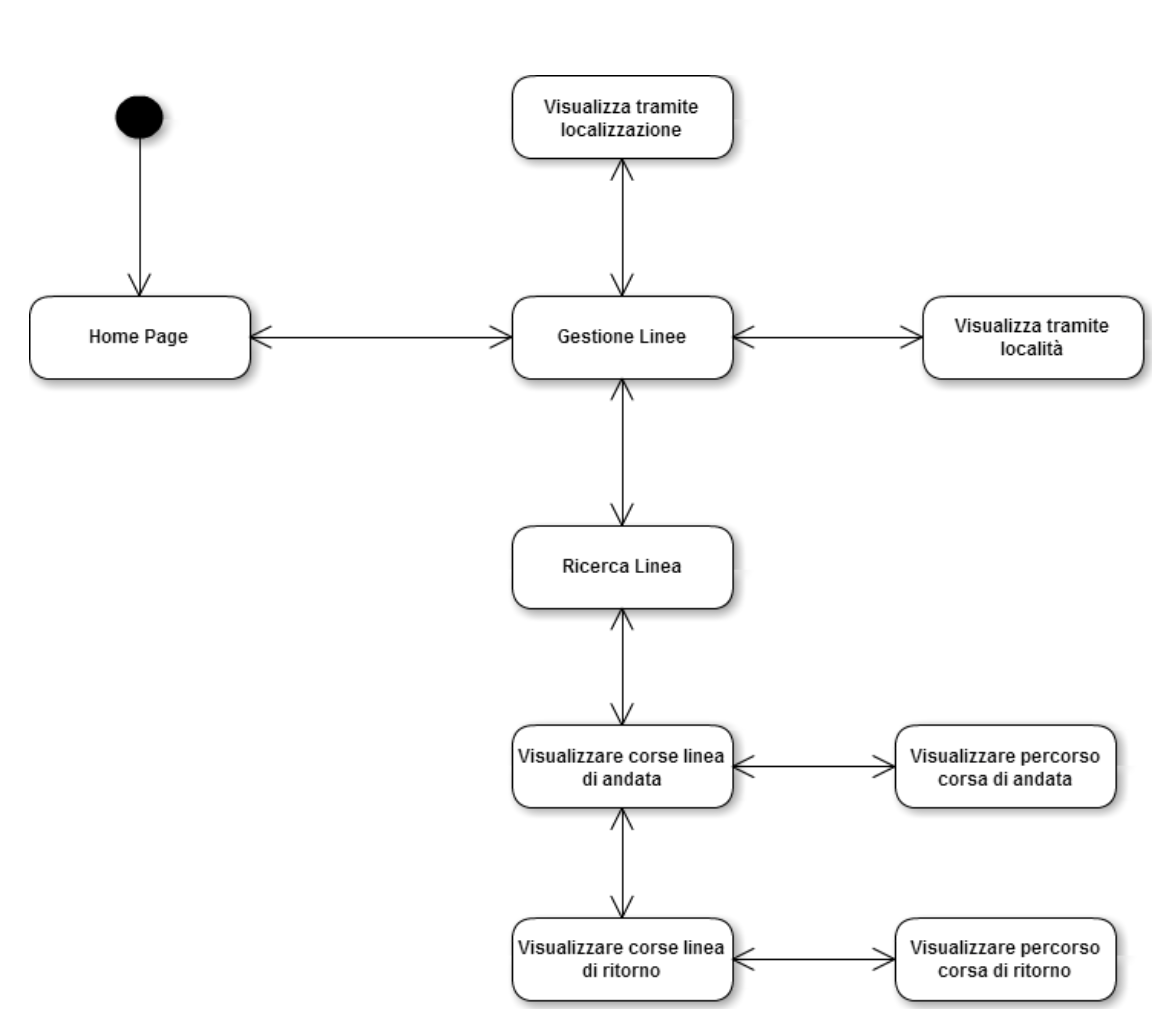
\includegraphics[scale=.4]{img/np.png}
\caption{Path navigazionale relativo alla gestione delle linee.}
\label{fig:np}
\end{figure} 

Come mostrato in Figura \ref{fig:np}, l'utente, a partire dalla Home Page dell'applicazione, pu\`{o} accedere alla funzionalit\`{a} di Gestione delle Linee, all\rq interno della quale pu\`{o} accedere:
\begin{itemize}
\item alla visualizzazione delle linee tramite geo-localizzazione;
\item alla ricerca di una linea.
\end{itemize}
Effettuando il caso d\rq uso mostrato in Figura \ref{fig:cd}, l\rq utente accede alla schermata di visualizzazione delle corse di andata per la linea selezionata, inoltre pu\`{o} visualizzare le corse di ritorno.\\

Infine, l'ultima parte dell\rq analisi dei requisiti \`{e} consistita nella definizione dei mockup delle funzionalit\`{a} identificate. In Figura \ref{fig:ui} \`{e} mostrato il mockup della funzionalit\`{a} di ricerca di una linea, implementato sulla base di una interfaccia per smartphone. 

\begin{figure}[h]
\centering
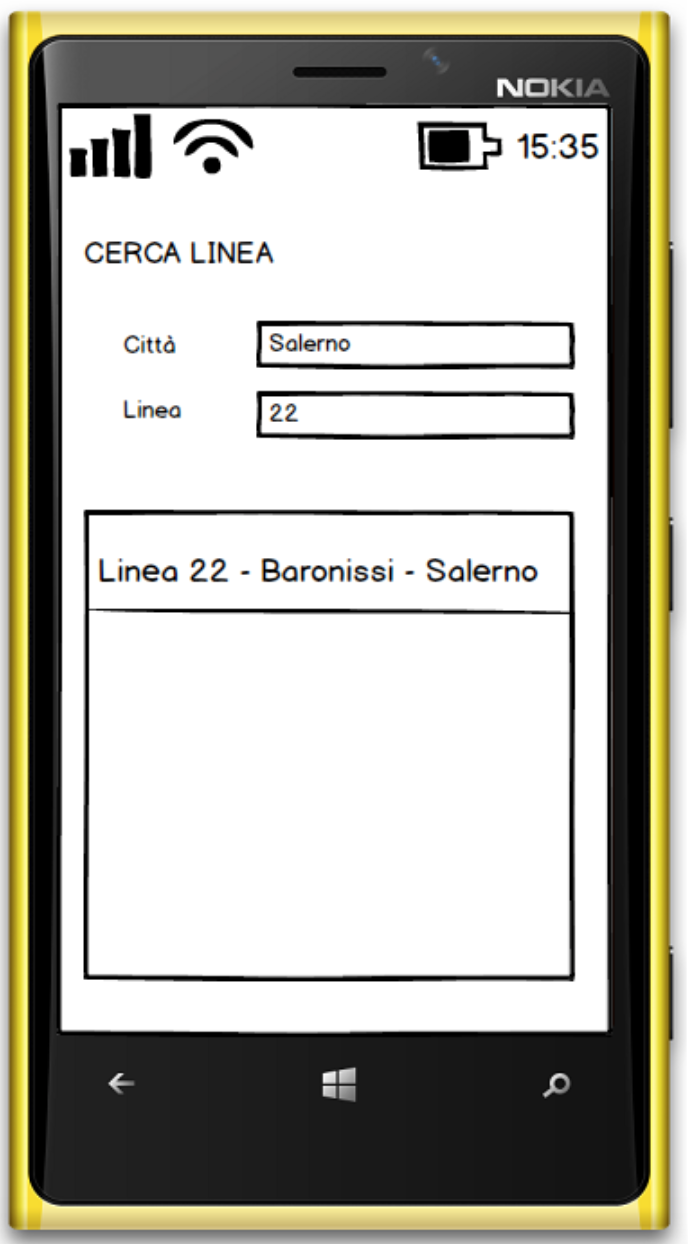
\includegraphics[scale=.3]{img/ui.png}
\caption{Screen Mockup della Funzionalit\`{a} di Ricerca di una Linea.}
\label{fig:ui}
\end{figure} 

La definizione degli screen mockup ci ha aiutato nella comprensione dei requisiti, ma anche nella definizione degli artefatti di basso livello descritti nelle successive sezioni. 

\subsection{Design}
Gli obiettivi principali della fase di design sono stati quelli di definire
\begin{itemize}
\item design goal;
\item architettura dell\rq applicazione;
\item mapping hardware-software.
\end{itemize}
Il primo step \`{e} consistito nella definizione degli obiettivi di design a partire dai requisiti non funzionali presenti nel documento di analisi e specifica dei requisiti. Sono stati identificate quattro categorie di design goal, di seguito riportati:\\

\noindent {\bf{DG-0 - Dependability criteria}}:  \emph{GoBus} garantir\`{a} il corretto svolgimento delle proprie funzioni, gestendo i vari errori logici (quelli derivanti da una negligenza da parte dell\rq utente), che potranno verificarsi durante l\rq utilizzo, ed eventuali attacchi alla sicurezza. Questo insieme di design goal comprende i requisiti di robustezza, affidabilit\`{a}, disponibilit\`{a} e sicurezza.\\

\noindent {\bf{DG-1 - Performance criteria}}:  Il sistema sar\`{a} usabile e leggero, in modo tale che, in caso più persone accedano al sistema contemporaneamente, questo non subisca rallentamenti. In definitiva, il sistema dovr\`{a} garantire che le varie operazioni offerte vengano svolte entro un intervallo di tempo accettabile. Questo insieme di design goal comprende i tempi di risposta, il throughput, e i requisiti di memoria.\\

\noindent {\bf{DG-2 - Maintenance criteria}}:  \emph{GoBus} garantir\`{a} un alto grado di manutenibilit\`{a}. Questo insieme di design goal comprende l\rq estendibilit\`{a}, la modificabilit\`{a} e la tracciabilit\`{a} dei requisiti.\\

\noindent {\bf{DG-3 - End User criteria}}:  \emph{GoBus} garantir\`{a} la learnability e l\rq usabilit\`{a} del sistema.\\

Per quanto riguarda l\rq architettura del sistema, \emph{GoBus} sar\`{a} implementato attraverso un'architettura three-tier, e quindi tramite una suddivisione del sistema in tre livelli:
\begin{itemize}
\item \emph{presentation-layer}, ovvero le interfacce grafiche che consentiranno all\rq utente di poter dialogare con la logica di business;
\item \emph{application-layer}, ovvero la logica applicativa del sistema;
\item \emph{storage-layer}, ovvero le componenti che consentono la memorizzazione dei dati.
\end{itemize}

Il passo successivo \`{e} consistito nella decomposizione del sistema in sottosistemi. In questo contesto, le metriche di coesione e accoppiamento rappresentano un importante strumento per poter definire una decomposizione che consenta a team di sviluppo separati di poter eseguire parallelamente diversi task. Nel nostro contesto, \`{e} stata definita la decomposizione mostrata in figura \ref{fig:sd}.

\begin{figure*}[tb]
\centering
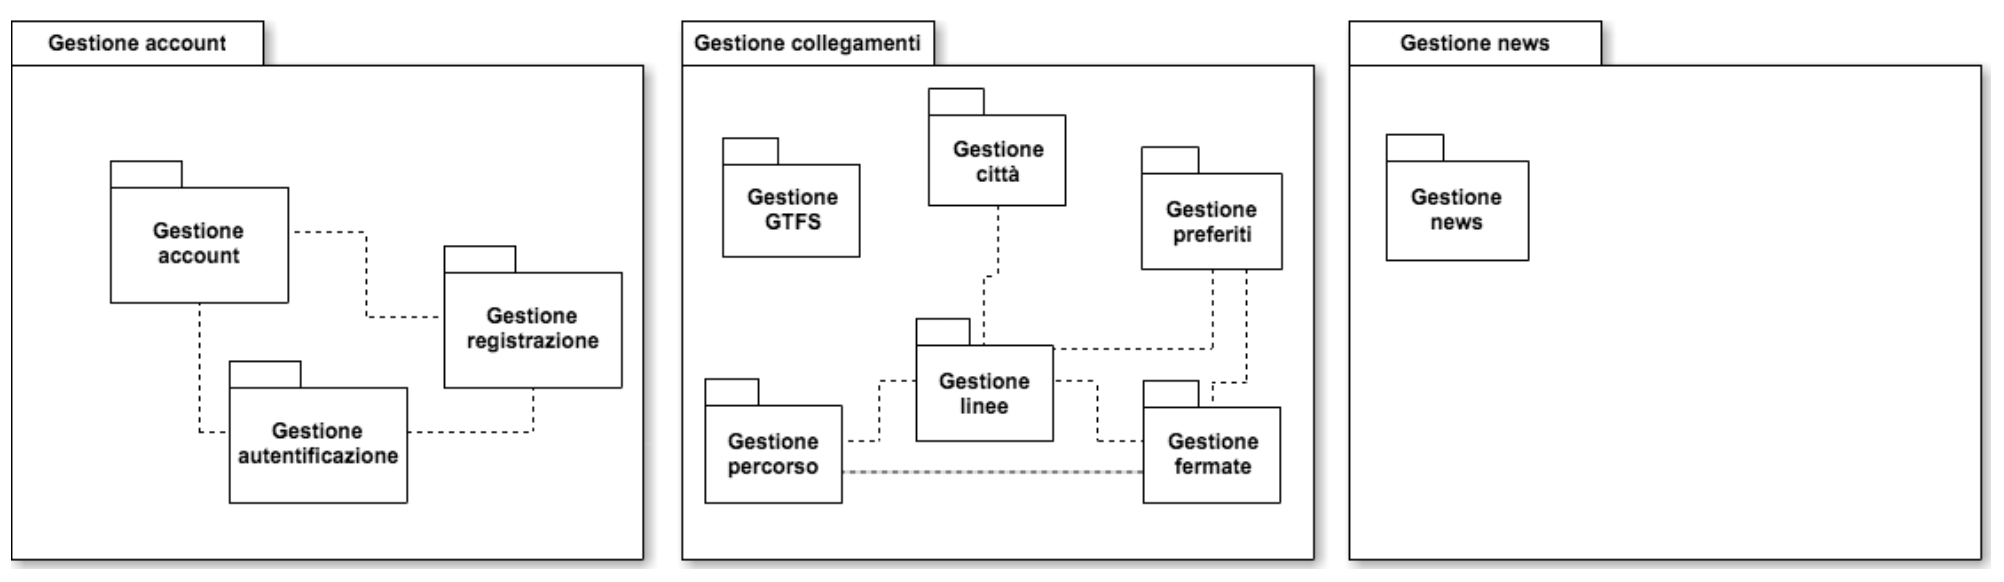
\includegraphics[scale=.4]{img/sd.png}
\caption{Decomposizione in Sottosistemi}
\label{fig:sd}
\end{figure*} 

Come \`{e} possibile vedere, \emph{GoBus} si compone di tre sottosistemi, che fanno riferimento a:
\begin{itemize}
\item gestione degli utenti;
\item gestione dei dati relativi alle fermate, alle linee e ai percorsi, inclusi i preferiti;
\item gestione delle notizie.
\end{itemize}

\begin{figure*}[tb]
\centering
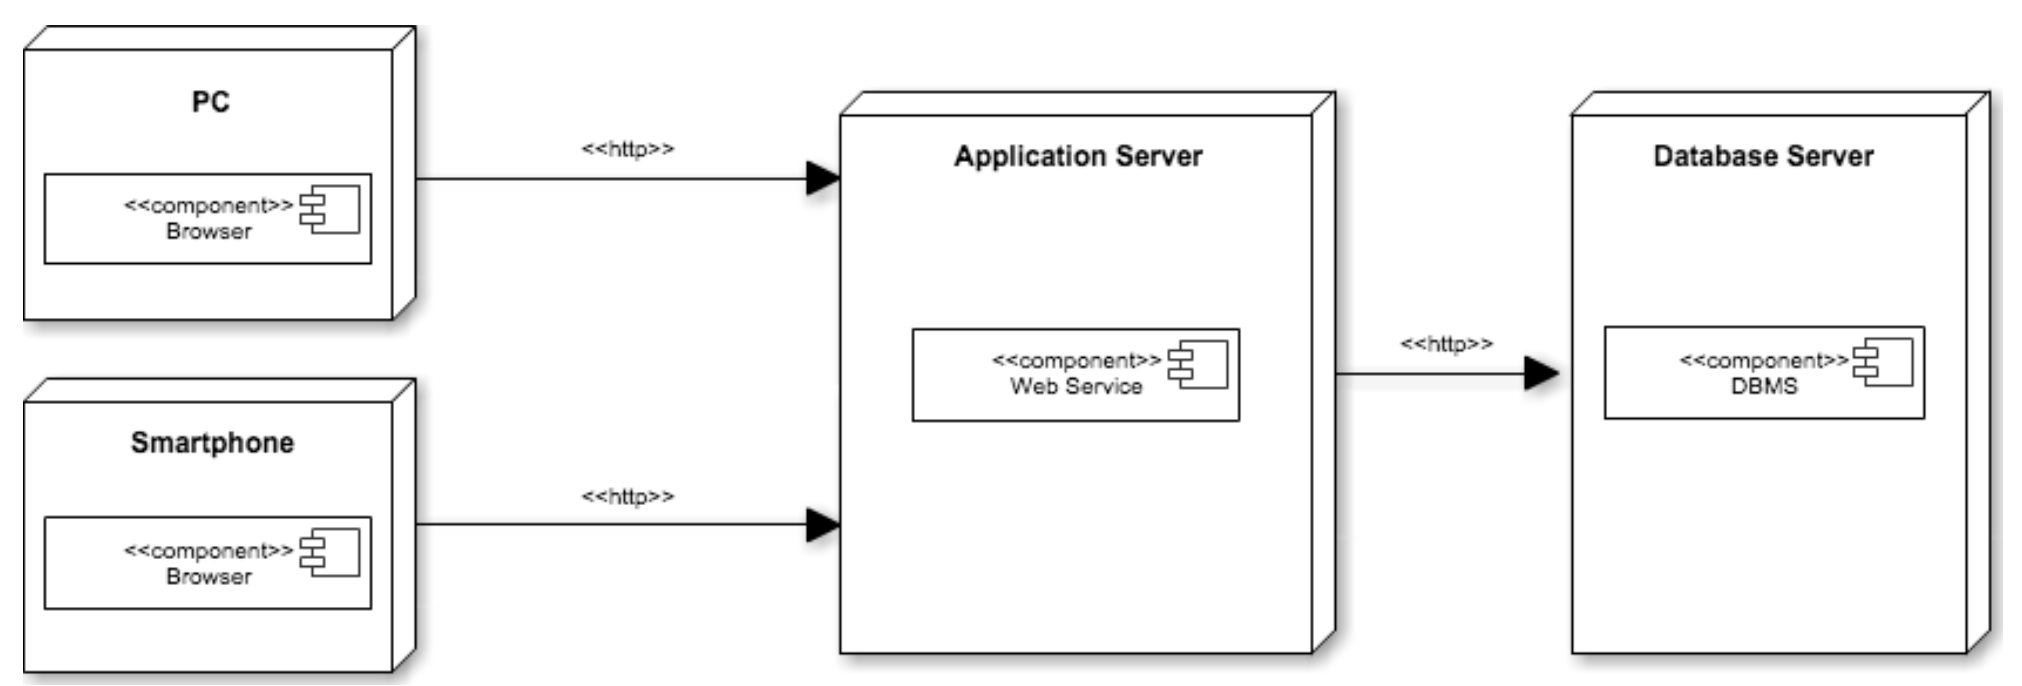
\includegraphics[scale=.4]{img/mhs.png}
\caption{Mapping Hardware/Software}
\label{fig:mhs}
\end{figure*} 

Infine, \`{e} stato definito il mapping hardware-software. Il Deployment Diagram fornisce un ausilio agli sviluppatori per quanto riguarda l\rq organizzazione delle componenti hardware e software del sistema \emph{GoBus}. In figura \ref{fig:mhs} possiamo vedere quali sono i nodi che interagiscono col sistema ovvero Application Server e Database Server. Le interfacce dei vari sottosistemi accedono ai pacchetti dell\rq Application Server, in cui risiedono gli oggetti di tipo control ed entity. L\rq accesso al database avviene tramite un sottosistema di storage, per garantire, anche, l\rq indipendenza da esso; infatti se sorgesse la necessit\`{a} di modificare una qualsiasi componente dell\rq interfaccia del sottosistema, non vi sarebbe il bisogno di apportare numerevoli modifiche all\rq interno del sistema. La comunicazione tra i nodi avviene tramite protocollo HTTP.\\
Per quanto riguarda la base di dati del progetto \`{e} stata modellata in base al formato General Transit Feed Specification Reference (GTFS). Questo formato \`{e} attualmente utilizzato dalle aziende di trasporto pubblico per la comunicazione dei dati, 
relativi ai servizi forniti, all\rq applicazione Google Transit. Questo consente alle aziende di fornire informazioni al progetto in modo facile e veloce, senza ridondanza di dati. Google fornisce le linee guida per la formattaione dei dati in questione, identificando un insieme di file. Tra questi ci sono file richiesti e file opzionali, ogni agenzia pu\`{o} decidere quali informazioni fornire in base alle proprie esigenze. \emph{GoBus} si propone di raggruppare  in un\rq unica applicazione informazioni su tutte le agenzie di trasporto nazionali, per cui  gestisce solo i dati obbligatori pi\`{u} alcune informazioni che non possono essere ignorate se fornite dall\rq agenzia, come ad esempio le eccezioni al calendario delle corse in giorni particolari. Questi file sono:\\

\begin{itemize}
\item {\bf{agency.txt}}: Uno o pi\`{u} agenzie di transito che forniscono i dati.\\
\item {\bf{stops.txt}}: Luoghi dove i bus fanno salire o scendere i passeggeri.\\
\item {\bf{routes.txt}}: Un percorso \`{e} un gruppo di viaggi che vengono visualizzati come un unico servizio.\\
\item {\bf{trips.txt}}: Viaggi per ogni itinerario. Un viaggio \`{e} una sequenza di due o pi\`{u} ferma relative ad un viaggio.\\
\item {\bf{stop\_ times.txt}}: Orario in cui un veicolo arriva ad una fermata, per ogni viaggio.\\
\item {\bf{calendar.txt}}: Date per i servizi che utilizzano un programma settimanale. Specifica quando viene avviato il servizio e finisce, oltre ai giorni della settimana in cui il servizio\`{e} disponibile.\\
\item {\bf{calendar\_ dates.txt}}: Date particolari in cui alcuni servizi subiscono una variazione.\\
\end{itemize}
All\rq interno degli stessi file, sono indicati dei campi obbligatori e dei campi opzionali.
Per comprendere la struttura della base di dati la \emph{figura 17} mostra il Diagramma Entit\`{a} Relazioni.



\begin{figure}[h]
\centering
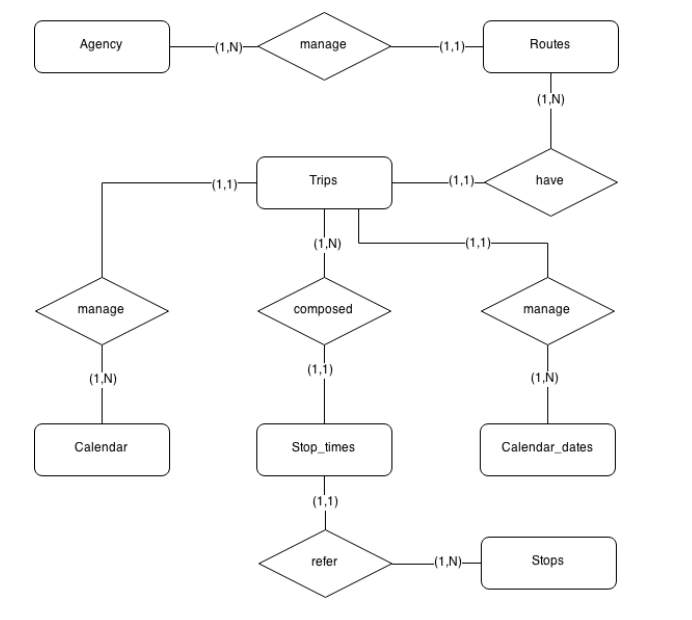
\includegraphics[scale=.4]{img/ER.png}
\caption{Diagramma Base di Dati}
\label{fig:ER}
\end{figure}

Infine, all\rq interno del design \`{e} stato analizzato il controllo degli accessi. 
Il dettaglio completo delle attivit\`{a} svolte in questa fase \`{e} nel documento di System Design allegato.

\subsection{Implementazione}
La fase di implementazione ha lo scopo di creare un prodotto software in grado di soddisfare tutti i requisiti individuati nela fase di pianificazione. Nell'ambito del progetto, tale attivit\`{a} viene svolta seguendo un modello evolutivo a prototipi. 

Il primo prototipo implementato ha lo scopo di comprendere al meglio i requisiti del web service e del portale web. In questa fase non \`{e} stato ritenuto necessario implementare il prototipo dell\rq applicazione mobile in quanto essa presenta gli stessi requisiti del portale web. 

In particolare il percorso di sviluppo \`{e} stato il seguente:\\
\begin{itemize}
\item Il web service \`{e} stato implementato in linguaggio php, con l\rq utilizzo di un framework esterno, Slim\footnote{http://www.slimframework.com}, il cui scopo \`{e} quello di mappare gli url inseriti dall\rq utente in query che presentino le informazioni dal database. In questo modo viene garantito che il web service utilizzi il protocollo rest. I risultati sono forniti in formato JSON (mostrata in \emph{figura 18}). \\
\item La web application \`{e} stata realizzata utilizzando Bootstrap\footnote{http://getbootstrap.com} e il framework jQuery\footnote{http://jquery.com}. Nel primo prototipo sono state implementate soltanto le funzionalit\`{a} principali, tralasciando la gestione dell\rq utente e degli avvisi (mostrata in \emph{figura 19}). \\
\end{itemize}

\begin{figure*}[tb]
\centering
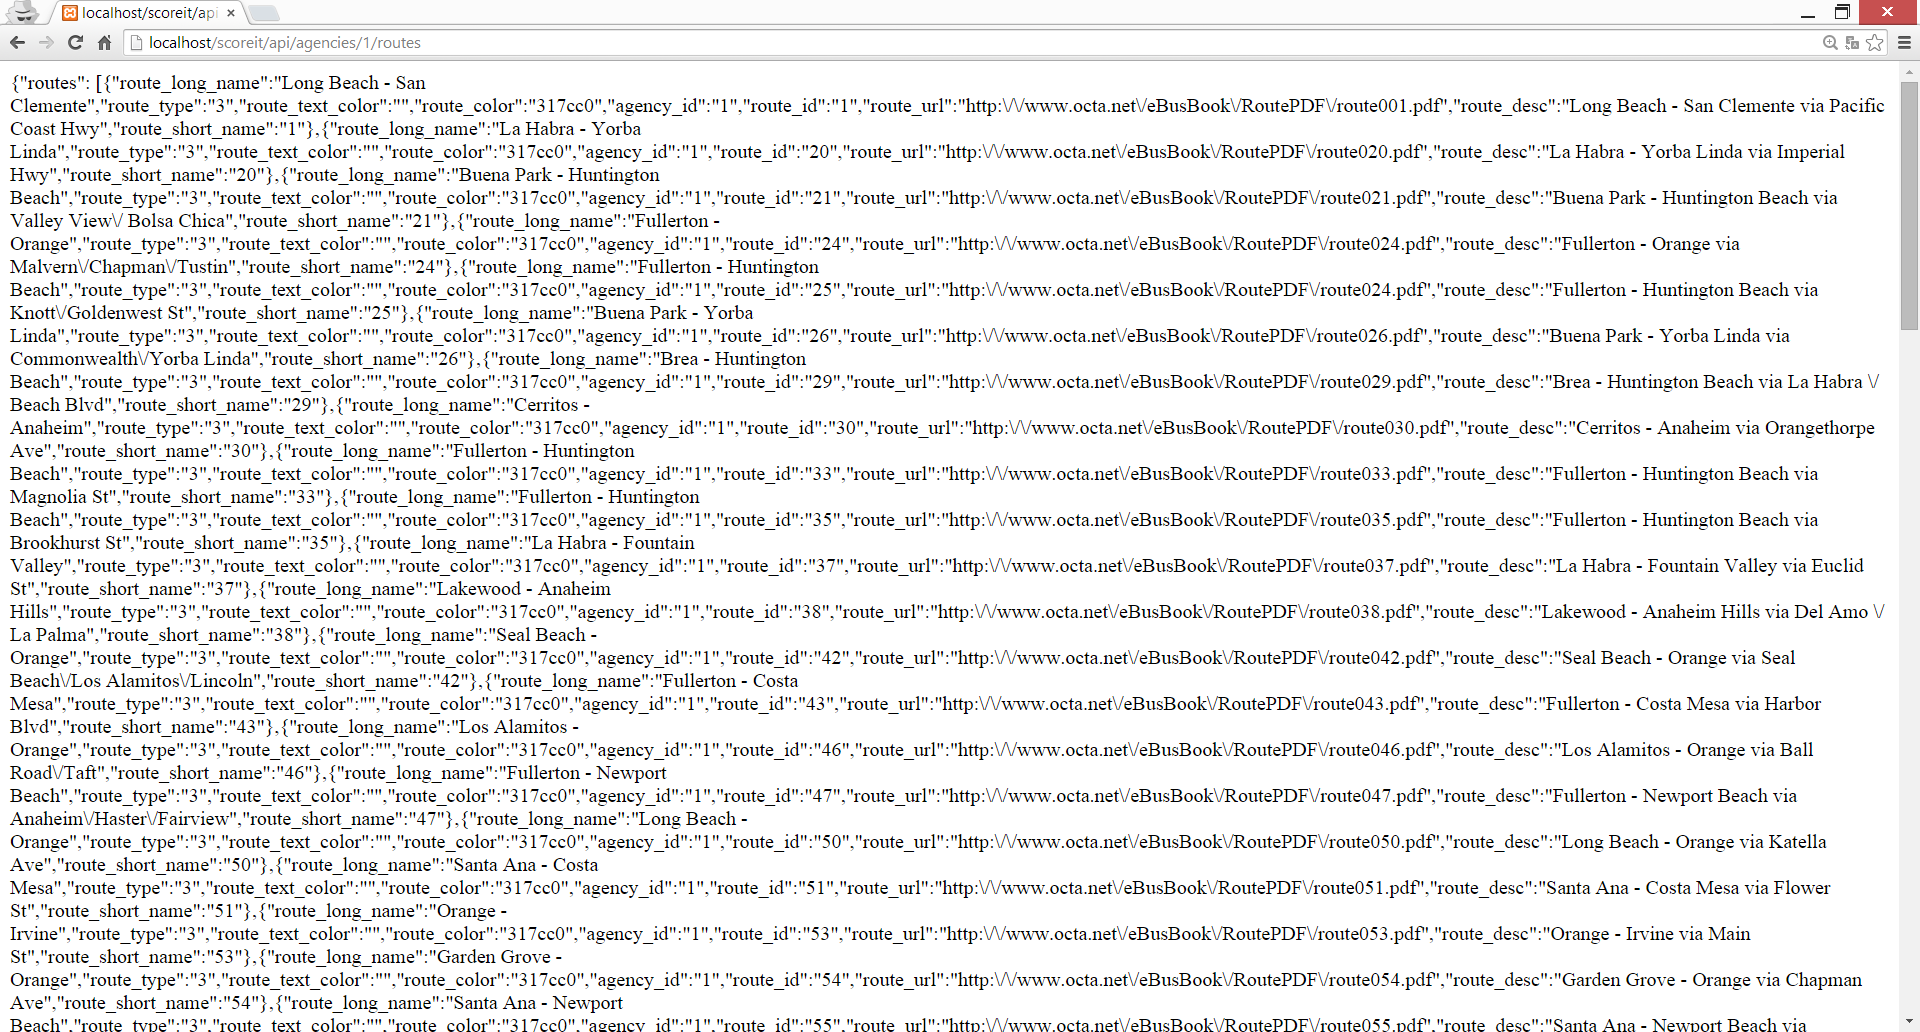
\includegraphics[scale=.3]{img/19.png}
\caption{Esempio risultato ricerca linea su Web service }
\label{fig:mhs}
\end{figure*} 

\begin{figure*}[tb]
\centering
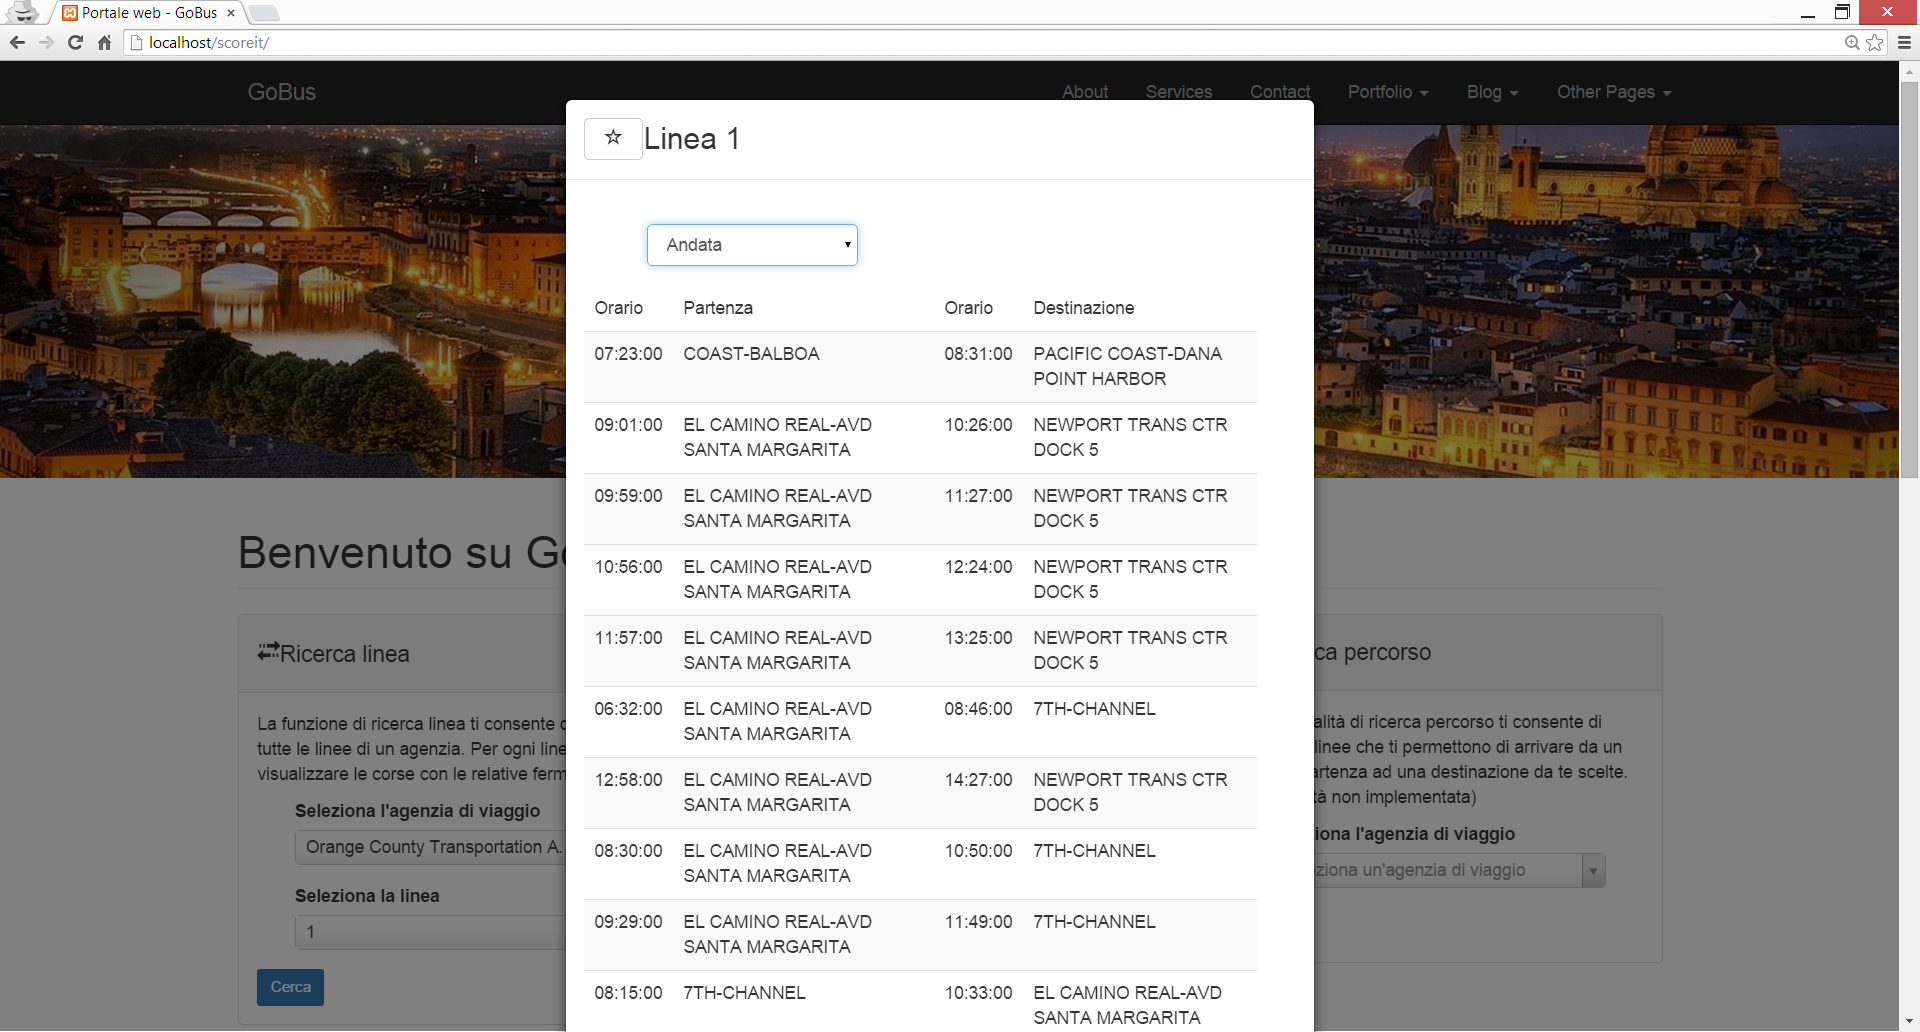
\includegraphics[scale=.3]{img/20.png}
\caption{Esempio risultato ricerca linea su Web application }
\label{fig:mhs}
\end{figure*} 

Il primo prototipo ha evidenziato di essere inefficiente in quanto alcune query rilevanti hanno mostrato tempi di risposta troppo elevati. A tal proposito sono state valutate diverse alternative, tra cui una diversa architettura della base di dati e l\rq utilizzo di un database ad oggetti come MongoDB\footnote{http://www.mongodb.org/ }. Tra le caratteristiche che suggeriscono l\rq adeguatezza di questo database si sottolineano l\rq architettura distribuita e la performance date dalla sua natura ad oggetti. Il portale web ha permesso di chiarire le modalit\`{a} di visualizzazione delle informazioni per quanto riguarda la gestione delle fermate e la gestione delle linee. 

\subsection{Testing}
La pianificazione del testing prevede tre tipologie di testing:
\begin{itemize}
\item testing di unit\`{a};
\item testing di integrazione;
\item testing di sistema.
\end{itemize}
In merito al testing di unit\`{a}, il processo di testing per il progetto "GoBus" verr\`{a} sottoposto ad una tipologia di testing di tipo black-box, ovvero, si stresser\`{a} il sistema dal punto di vista funzionale, analizzando e confrontando gli output derivanti dagli input immessi, con gli output attesi. In combinazione con il testing black-box sar\`{a} utilizzato category partition. Questa tecnica permette di dividere i possibili input in gruppi, i cui elementi generano output logicamente simili. Tali gruppi, identificati come classi di equivalenza, saranno identificati e utilizzati in modo da eseguire almeno un test per ognuno di essi. Per agevolare il testing di regressione, in seguito alla modifica delle componenti software verr\`{a} utilizzato un framework adatto.\\
Relativamente al testing di integrazione, verr\`{a} adottata una strategia di tipo bottom-up. In sintesi si testeranno le componenti del sistema partendo dal layer pi\`{u} in basso nella gerarchia. L\rq implementazione di tale strategia prevede la costruire di driver test, ovvero di classi che utilizzino in maniera banale le componenti sotto test.\\
Il testing di sistema verr\`{a} effettuato mediante l\rq analisi empirica statica, ovvero confrontando il comportamento del sistema in esecuzione in relazione al comportamento atteso.\\

\begin{figure}[h]
\centering
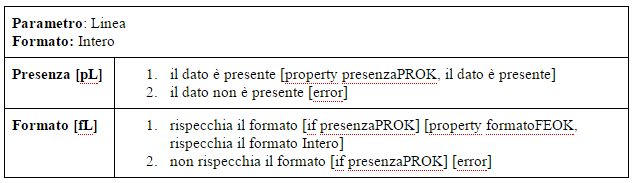
\includegraphics[scale=.5]{img/21.png}
\caption{Esempio Test case }
\label{fig:mhs}
\end{figure}  

\begin{figure}[h]
\centering
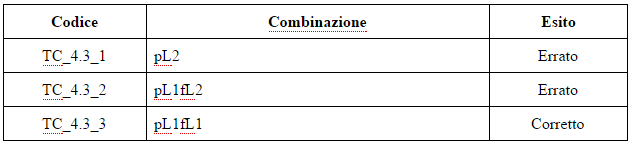
\includegraphics[scale=.5]{img/22.png}
\caption{Esempio combinazione Test}
\label{fig:mhs}
\end{figure} 

\begin{figure}[h]
\centering
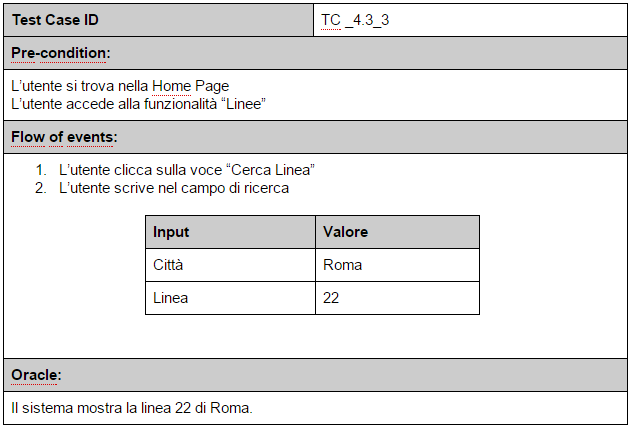
\includegraphics[scale=.5]{img/23.png}
\caption{Esempio category partition }
\label{fig:mhs}
\end{figure} 

\subsection{Rilascio}
Il prototipo \`{e} stato rilasciato. Per maggiori informazioni, si pu\`{o} fare riferimento al file zip contenente il codice dell\rq implementazione, disponibile in allegato, e al video che mostra la demo dell\rq applicazione, disponibile su Youtube all\rq indirizzo http://tinyurl.com/kareo9e .
